\begin{figure}[H]
    \centering
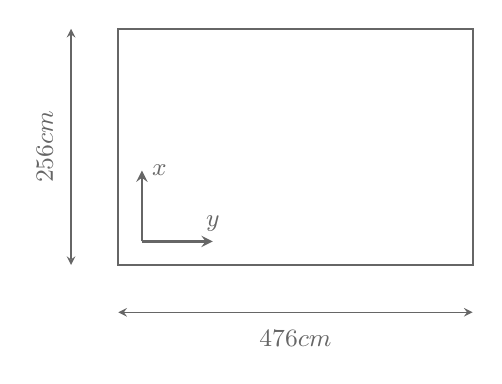
\begin{tikzpicture}[
    scale=1.5,
    cota/.style={<->, >=stealth, thin, gray!80!black},  % Estilo das linhas de cota
    retangulo/.style={draw=gray!80!black, thick},% Estilo do retângulo
    eixo/.style={->, >=stealth, thick, gray!80!black}   % Estilo dos eixos x e y
]

    % 1. Coordenadas do retângulo
    \coordinate (A) at (0, 0);
    \coordinate (B) at (3, 0);
    \coordinate (C) at (3, 2);
    \coordinate (D) at (0, 2);

    % 2. Desenho do Retângulo
    \draw[retangulo] (A) rectangle (C);

    % 3. Eixos de Coordenadas x e y (Origem no canto inferior esquerdo, dentro do retângulo)
    \draw[eixo] (0.2, 0.2) -- (0.8, 0.2) node[above, font=\small\bfseries] {$y$};
    \draw[eixo] (0.2, 0.2) -- (0.2, 0.8) node[right, font=\small\bfseries] {$x$};

    % --- COTA HORIZONTAL (Texto abaixo da linha) ---
    \def\offsetH{0.4}
    \draw[cota] (0, -\offsetH) -- (3, -\offsetH) 
        node[midway, below=3pt, font=\small] {$476\text{ cm}$};

    % --- COTA VERTICAL (Texto à esquerda da linha) ---
    \def\offsetV{0.4}
    \draw[cota] (-\offsetV, 0) -- (-\offsetV, 2) 
        node[midway, left=3pt, font=\small, rotate=90, anchor=south] {$256 \text{ cm}$};

\end{tikzpicture}
    %\caption{Caption}
    %\label{fig:placeholder}
\end{figure}